% Fakesection 序言之前

\RequirePackage[l2tabu, orthodox]{nag}
\RequirePackage{ifxetex}
\RequireXeTeX

\ifnum\strcmp{\jobname}{handout}=0
	\documentclass[handout]{ctexbeamer}
\else
	\documentclass{ctexbeamer}
\fi

%颜色
\usepackage{xcolor}

%长度
\usepackage{printlen}
\uselengthunit{mm}

%图形
\usepackage{media9}
\usepackage{pdfpages}
\usepackage{overpic}
\usepackage{graphicx}
\graphicspath{{./src/}}
\usepackage{wallpaper}
\usepackage{wrapfig}
\usepackage{pstricks}
\usepackage{smartdiagram}
\usepackage[edges]{forest}
\usepackage{pgfplots}
\usepackage{tikz}
\usetikzlibrary{shapes.geometric}
\usetikzlibrary{calc}
\usetikzlibrary{patterns}
\usetikzlibrary{arrows}
\usetikzlibrary{shapes}
\usetikzlibrary{chains}
\usetikzlibrary{mindmap}
\usetikzlibrary{graphs}
\usetikzlibrary{decorations.text}
\usetikzlibrary{arrows.meta}
\usetikzlibrary{shadows.blur}
\usetikzlibrary{shadings}
\usepackage{scsnowman}
\usepackage{tikzpeople}
\usepackage{tikzducks}
\usepackage{fontawesome}
\usepackage{ean13isbn}
\usepackage{qrcode}
\usepackage{pgf-pie}
\usepackage{pgfmath}

%表格
\usepackage{tabu}
\usepackage{longtable}
\usepackage{booktabs}
\usepackage{diagbox}
\usepackage{multicol}
\usepackage{multirow}
\usepackage{makecell}
\usepackage{fancybox}
\usepackage{colortbl}
\usepackage{tcolorbox}
\tcbuselibrary{skins}
\tcbuselibrary{breakable}
\tcbuselibrary{theorems}
\tcbuselibrary{listings}
\tcbuselibrary{xparse}
\tcbuselibrary{minted}% 用minted排版代码
\usepackage{fvextra}
\usepackage{csvsimple}
\usepackage{boxedminipage2e}

%公式
\usepackage{amsmath}
\usepackage{amsthm}
\usepackage{amsfonts}
\usepackage{amssymb}
\usepackage{amsbsy}
\usepackage{amsopn}
\usepackage{amstext}
\usepackage{mathrsfs}
\usepackage{bm}
\usepackage{textcomp}
\usepackage{latexsym}
\usepackage{exscale}
\usepackage{relsize}
%\usepackage{xymtex}
\usepackage{physics}
\usepackage{siunitx}
\usepackage{hologo}
\usepackage{cases}

%正文
\usepackage{fancyhdr}
\usepackage{geometry}
\usepackage{lastpage}
\usepackage{indentfirst}
\usepackage{setspace}
\renewcommand\arraystretch{1.5}

%非正文
\usepackage{makeidx}
\makeindex
\usepackage{epigraph}
\usepackage{varwidth}

%参考文献
\usepackage{morewrites}
\renewcommand{\thefootnote}{\fnsymbol{footnote}}
\usepackage[resetlabels]{multibib}

%标题
\usepackage{caption}
\usepackage{subcaption}

%其它
\usepackage{atbegshi}
\usepackage{lipsum}

%文字
\usepackage{csquotes}
\usepackage{microtype}

\csname
endofdump
\endcsname

%\usepackage[notref,notcite]{showkeys}

%代码
\usepackage{minted}
%Java %与mcode冲突
% \usepackage{lstcustom}
%Matlab %与lstcustom冲突
%\usepackage[framed,numbered,autolinebreaks,useliterate]{mcode}
%\usepackage{boxie}
%\makeatletter
%\xdefinecolor{tcbcol@back}{rgb}{0,0,0}
%\makeatother

\usetheme{Xiaoshan}
%\metroset{progressbar=none}
\usepackage{pgfpages}
\ifnum\strcmp{\jobname}{main}=0
	\setbeameroption{show notes on second screen = right}
\fi

\begin{document}

% Fakesection 扉页

\title{\textbf{铱星陨落之因}}
\subtitle{铱星计划案例分析}
\author{吴振宇~董浩宸\\沈树民~刘金岩}
\institute{南京理工大学\\经济管理学院}
\date{\today}
\titlegraphic{%
	\includegraphics[width=.5\linewidth]{njust.ai}
	\vspace{4.5cm}
	\begin{flushright}
		\qrcode[hyperlink, height=1.6cm]{https://github.com/Freed-Wu/}
	\end{flushright}
}
\maketitle

\section{案例简介}%
\label{sec:案例简介}

\begin{frame}{公司简介}
	\begin{columns}
		\begin{column}{0.5\textwidth}
			\begin{itemize}
				\item 摩托罗拉 \footnote{(Motorola Inc )} ,是一家总部设在美国伊利诺伊州绍姆堡,位于芝加哥市郊。世界财富百强企业之一,是全球芯片制造、电子通讯的领导者。主要经营业务有消费电子、移动通信、互联网等,产品有通讯产品、网络产品、软件等。
			\end{itemize}
		\end{column}
		\pause
		\begin{column}{0.5\textwidth}
			\begin{figure}[htpb]
				\centering
				
\includegraphics[width=0.8\linewidth]{motorola.jpg}
				\caption{摩托罗拉公司}
				\label{fig:摩托罗拉公司}
			\end{figure}
		\end{column}
	\end{columns}
	\cite{2016企业战略与风险管理}
\end{frame}

\begin{frame}{由盛转衰}
	\begin{columns}
		\begin{column}{0.5\textwidth}
			\begin{itemize}
				\item 在1995年摩托罗拉在中国的市场占有率高达60\%以上,而仅仅过去了10年,就已经跌至12\%不到。思考其原由不由令人唏嘘。\cite{吴定祥2015中国联想并购摩托罗拉案例分析}
			\end{itemize}
		\end{column}
		\pause
		\begin{column}{0.5\textwidth}
			\begin{figure}[htpb]
				\centering
				\begin{tikzpicture}[scale=.5]
					\begin{axis}[ybar,enlargelimits=0.15]  % 绘制关于y坐标的条形图,条形之间的最大间隔是0.15cm
						\addplot[draw=blue,fill=red]           % 蓝色边界、红色填充
							coordinates
							{
								(1,99.93) (2,94.09) (3,89.63) (4,88.81)
							};
						\addplot[draw=black,fill=blue]         % 黑色边界、蓝色填充
							coordinates
							{
								(1,110.83) (2, 106.85) (3, 103.58) (4, 103.73)
							};
						\addlegendentry{资产/负债 (亿) };
					\end{axis}
				\end{tikzpicture}
				\caption{各季度资产/负债}
				\label{fig:各季度资产/负债}
			\end{figure}
		\end{column}
	\end{columns}
	\note{根据资产负债表,可见负债的规模正在逐年增长,负债方面存在着比较大的上升\%。企业负债规模会影响企业的发展,显而易见,企业负债规模过大,就会产生企业利息支出增大的问题,企业的收益也会相应的减少,偿付能力就会减弱,使得筹资风险增大。在企业的总负债当中,由于长期和短期负债占比不可能完全相同,缺乏合理安排长期负债的比例,增加了企业融资的风险。资产规模也在逐年增长,企业偿还债务的能力逐年减弱,存在一定的财务风险。}
\end{frame}

\begin{frame}{项目简介}
	\begin{columns}
		\begin{column}{0.5\textwidth}
			\begin{itemize}
				\item 为了夺得对世界移动通信市场的主动权,并实现在世界任何地方使用无线手机通信,以摩托罗拉为首的美国一些公司在政府的帮助下,于 1987 年提出新一代卫星移动通信星座系统——铱星。由66颗近地卫星组成的星群,让用户从世界上任何地方都可以打电话。
					\note{铱星计划从现代电信系统设计的角度来看, 是一个符合市场需求的系统。 它在总体技术上采用了大量以往的卫星通信系统所未曾采用过的新技术, 使得相对传统的基于地球静止轨道的全球移动通信系统而言, 铱星移动通信系统在性能、 经济、 时间和发展等四个方面都达到和保持良好状态, 并取得了非常强的竞争优势。 铱星系统是世界上第一个投入使用的大型低地球轨道移动的通信卫星系统, 在实际进入工程建设的几个移动通信卫星星座中, 铱星系统技术是最先进、星座规模最大、投资最多、建设速度最快的。从理论上讲,铱星占尽了市场的先机, 开创了全球个人通信的新时代,使人们在地球上任何“能见到天的地方”都可以进行“无缝隙”的通信联络。它实现了 5 个“任何”(即 5W) :即任何人在任何地点、任何时间与任何人采取任何方式进行通信,被认为是现代通信的一个里程碑。}
			\end{itemize}
		\end{column}
		\pause
		\begin{column}{0.5\textwidth}
			\begin{figure}[htpb]
				\centering
				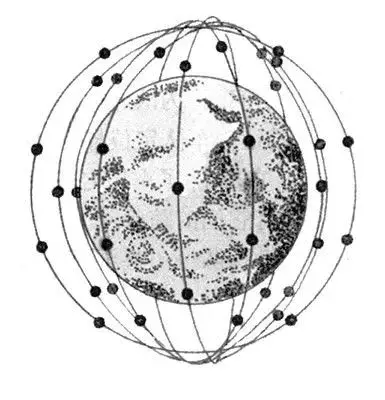
\includegraphics[width=0.8\linewidth]{77.png}
				\caption{铱星计划}
				\label{fig:铱星计划}
			\end{figure}
		\end{column}
	\end{columns}
\end{frame}

\begin{frame}{项目初期}
	\begin{block}{名声广传}
		\begin{itemize}
			\item 投入 1亿美元进行广告宣传;
			\item 每股股价从发行时的 20 美元飙升到 1998 年 5 月的 70 美元。
		\end{itemize}
	\end{block}
	\pause
	\begin{block}{普遍看好}
		\begin{itemize}
			\item 1998 年被美雕大众科学杂志评为年度全球最佳产品之一,在由中国两院院士评选的年度十大科技成就中名列第二位;
			\item 媒体赞誉:世界上第八大奇迹、人类交流沟通方式中一个里程碑式的革命;
			\item 比尔· 盖茨产生了投资铱星的念头。
		\end{itemize}
		\note{媒体的追捧,科学家的褒扬,用户的欢呼,使得铱星的光环越来越亮。}
	\end{block}
\end{frame}

\begin{frame}[standout]
	然而,2000年3月,铱星公司背负40多亿美元债务破产了!
\end{frame}

\section{案例分析}%
\label{sec:案例分析}

\begin{frame}{SWOT 分析}
	\begin{figure}[htpb]
		\centering
		\begin{tikzpicture}[
			start chain=going right,
			node distance=5mm,
			every on chain/.style={
				thick,
				draw=black,
				top color=white,
				bottom color=yellow!40,
				font=\sffamily\small,
				minimum width=6mm,
				minimum height=6mm,
				%drop shadow,
				%label={below:block \tikzchaincount},
			},
			decoration={coil},
			dna/.style={decorate, thick, decoration={aspect=0, segment length=5cm}},
			%    post join/.style={
			%      -stealth,
			%      line width=1.5mm,
			%      red,
			%      rounded corners=1mm,
			%    },
			square/.style={thick,
				draw=black,
				top color=white,
				bottom color=black!10,
				font=\sffamily\small,
				minimum width=12mm,
				minimum height=10mm,
			drop shadow},
			every label/.style={
				font=\sffamily\scriptsize
			},
			]
			\draw[dna, decoration={amplitude=.15cm}] (0,-0) -- (1.1,-0);
			\draw[dna, decoration={amplitude=.35cm}] (1.15,0) -- (1.15,-1.1);
			\draw[dna, decoration={amplitude=.35cm}] (1.15,-1.1) -- (0,-1.1);
			\draw[dna, decoration={amplitude=.35cm}] (0,-1.1) -- (0,0);
			%% Path for dots
			\node [on chain] {优势};
			\node [on chain] {劣势};
			\node [on chain=going below] {机会};
			\node [on chain=going left] {威胁};
		\end{tikzpicture}
		\caption{SWOT模型}
		\label{fig:SWOT模型}
	\end{figure}
	\begin{itemize}
		\item 下面运用SWOT 模型对该战略进行分析。
	\end{itemize}
\end{frame}

\begin{frame}{优点}
	\begin{exampleblock}{优点}
		\begin{description}
			\pause
		\item[技术先进]采用了大量以往的卫星通信系统所未曾采用过的新技术,在性能、经济、时间和发展等四个方面,相对传统的基于地球静止轨道的全球移动通信系统,都达到和保持良好状态,并取得了非常强的竞争优势;
			\pause
		\item[占尽先机]开创了全球个人通信的新时代,实现了5个\enquote{任何}(即5W):即任何人在任何地点、任何时间与任何人采取任何方式进行通信。
	\end{description}
\end{exampleblock}
\end{frame}

\begin{frame}{缺点}
	\begin{alertblock}{缺点}
		\begin{description}
			\pause
		\item[脱离实际]相对地面移动电话系统,铱星手机个头笨重,运行不稳定,价格昂贵,不能在室内和车内使用;\note{整个世界通信系统的趋势却是手机越做越小,商家为了赚取通话费,甚至无偿赠送手机。}
			\pause
		\item[运营问题]原公司总裁爱德华·斯泰亚诺在营销和运作上出现了一系列失误,如在铱星系统投入商业运营时未能向零售商们供应铱星电话机,这也让它损失了不少用户。\note{据说公司的计划是初期中国的用户就要达到10万,可事实是不到1000个。}
	\end{description}
\end{alertblock}
\end{frame}

\begin{frame}{机会}
	\begin{exampleblock}{机会}
		\begin{description}
			\pause
		\item[偏远地区]那些身处偏远地方, 地面无线通信网无法延伸的地方, 如海上石油钻井平台或油轮上工作的人;
			\pause
		\item[稳定通信]大企业希望随时随地保持稳定通信对铱星计划有足够的兴趣。
	\end{description}
\end{exampleblock}
\end{frame}

\begin{frame}{威胁}
	\begin{alertblock}{威胁}
		\begin{description}
			\pause
		\item[地面通信]过去十年里地面移动通信发展迅猛,夺走了铱星公司的目标市场,相对地面移动通信,尤其是移动电话领域,铱星计划在时间维上已经失去了市场机会。
	\end{description}
\end{alertblock}
\end{frame}

\section{案例总结}%
\label{sec:案例总结}

\begin{frame}{经验教训}
	\begin{itemize}
		\pause
	\item 好的运营和管理的架构是正确决策的先机;\note{董事会28个成员说的是多国语言,每次开会就象是出席一次小型联合国会议,人人必须带着耳塞,收听5种语言的同步翻译;很多合伙人严重缺乏电讯业经验,比如委内瑞拉的投资者除了从事手机业务之外,还经营着奶制品。}
		\pause
	\item 对用户定位和数量的正确估计很重要;\note{认为用户都属于“付钱不看账单的一群人”的高层次的国际商务旅行人员。到申请破产为止,这个耗资50亿美元建立的通信网只有5.5万用户,而一些分析家估计该公司要实现盈利平衡至少需要65万用户。}
		\pause
	\item \alert{工程师的创意不能与市场现实脱轨!}\note{地面移动电话系统无论是技术还是市场都有雄厚的根基。}
\end{itemize}
\end{frame}

\begin{frame}{完}
	\begin{columns}
		\begin{column}{.7\textwidth}
			\begin{block}{参考}
				\bibliographystyle{IEEEtran}
				\bibliography{src/main}
			\end{block}

			\begin{block}{致谢}
				\begin{itemize}
					\item 老师的评审及意见;
					\item 台下同学的聆听和指正。
				\end{itemize}
			\end{block}
		\end{column}
		\begin{column}{.3\textwidth}
			\centering
			\ifnum\strcmp{\jobname}{titlepage}=0
				\else
					\includegraphics[width=\linewidth]{titlepage.pdf}
				\fi
			\end{column}
		\end{columns}
	\end{frame}

	\end{document}
